\documentclass{article}
\usepackage[T1,T2A]{fontenc}
\usepackage[utf8x]{inputenc}
\usepackage[english,russian]{babel}
\usepackage{amssymb,amsmath,geometry}
\usepackage{graphicx, caption}
\usepackage{wrapfig}
\usepackage{setspace}
\usepackage[usenames]{color}
\usepackage{colortbl}
\usepackage{indentfirst}

\geometry{top=4em,right=3em,left=3em,bottom=4em}

\begin{document}
\setlength\parindent{24pt}
\pagestyle{empty}
\newcommand{\Mainclt}{\raisebox{0pt}[\headheight][15pt]{\vbox{\hbox to\textwidth{\hfilЗАДАЧНИК <<КВАНТА>> \hfil29}}}}
\renewcommand{\footnoterule}{\vspace*{10pt}
\hrule width .4\columnwidth
\vspace*{=2.6pt}$^1$См.<<Алгебру>> Ван-дер-Вардена или другой учебник, где рассматривается <<многочлены деления круга>>}
\Mainclt
\setstretch{0.9}{
  \begin{minipage}[t]{0.47\textwidth}
    
    {\bfseries Лемма}. \slshapeПусть KLN - правильный треугольник, M - любая точка плоскости. Тогда \\
    \[{MN \le MK + ML..., .} \eqno (2)\]
    причем MN = MK + ML в том и только том случае, если M лежит на дуге описанной окружности,
    где ${\angle}KML = 120^{\circ}.$\upshape
    \begin{center}
      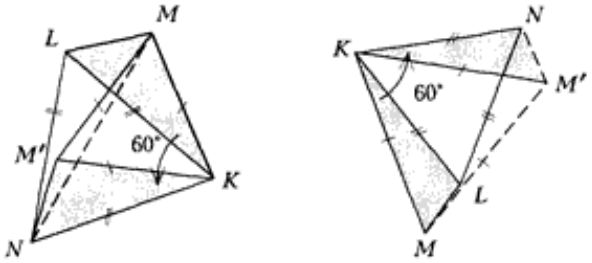
\includegraphics[width=0.9\textwidth]{src/painting1.png}
      \captionof{figure}{}
    \end{center}  
    Доказательство (рис.1). Повернём ${\vartriangle}KML$ вокруг точки $K$ на $60^{\circ}$ так, чтобы $L$ совпала с $N$. Пусть при этом повороте точка $M$ переходит в $M'$.
    Треугольник $KMM'$ правильный, поэтому $MM' + M'N = MK + ML$.
    Точка $M'$ лежит на отрезке $MN$ в том и только том случае, если ${\angle}KM'N = {\angle}KML = 120^{\circ}$ и $M$ лежит вне ${\vartriangle}KNL$.\\
    \slshapeЗамечание\upshape. Из решения ясно, что существует единственный "паук", для которого достигается равенство:
    за $H'$ и $G'$ надо взять точки пересечения $CF$ с описанными окружностями треугольников $AEF$ и $BCD$.
    \begin{center}\hfillН.Васильев\end{center}
    М1530. \slshapeПусть p - нечетное простое число. Найдите количество подмножеств А множества {1, 2, ..., 2p} таких, что\\
    (i)A содержит ровно p элементов;\\
    (ii)сумма всех элементов из A делится на p.\\
    \upshape
    Запись $a$ = $b$ всюду ниже означает, что разность $a$ - $b$ делится на $p$.
    Мы докажем, что ответ в задаче таков:
    \[
      (C^p_{2p} - 2)/p+2,
    \] где ${C^p_{2p} = (2p)!/(p!)^2}$ - число всех подмножеств из $p$ элементов множества из 2$p$ элементов.\\
    Приведём два разных доказательства.\\
    Первое более элементарно.\\
    Разобьем все $p$ - элементарные подмножества $A$ множества {1, 2, ..., $p$, $p + 1$, ..., $2p$}, отличные от <<наименьшего>> $B$ = {1, 2, ..., $p$} и <<наибольшего>> $С$ = {$p + 1$, ..., $2p$}, на группы по $p$ подмножеств в каждой, следующим образом. Ясно, что если $A \ne B$ и $A \ne C$, то $A \cap B$ и $A \cap C$ непусты.
    Два подмножества $A$ и $A'$ отнесем к одной группе, если $A \cap C = A' \cap C и A' \cap B$ получается из $A \cap B$ <<циклическим сдвигом>> по модулю $p$, т.е. если существует $m$, 0 < $m$ < $p$, такое что $x \in A \cap B \Leftrightarrow y = x + m \in A' \cap B$.
    Ясно, что кроме $A$ в ту же группу попадут еще $p - 1$ подмножеств. Обозначим через $s(A)$ сумму элементов в $A$. Пусть $A \cap B$  состоит из $q$ элементов; $q$ одно и то же для всех $A'$ из той же группы, что $A$, причем $s(A') - s(A) = mq$ не делится на $p$, если $A' \ne A$.
    Поэтому в каждой группе найдется ровно одно подмножество $A$, для которого $s(A) = 0$, Остается заметить, что $s(B) = s(C) = 0$ и что число групп равно $(C^p_{2p}-2)/p)$.
  \end{minipage}
  \hfill
  \begin{minipage}[t]{0.5\textwidth}
    Второе доказательство еще красивее, но требует знания комплексных чисел и нетривиальных теорем о многочленах.\\
    Пусть $\lambda$ - один из примитивных корней $p$-й степени из 1, например, $\lambda = \cos(2\pi/p)+i\sin(2\pi/p)$.\\
    Найдем сумму
    \[
      \sigma = \sum\lambda^{i_1+...+i_p}=\sum_{j=0}^{p-1}{n_j\lambda^j}\eqno(1)
    \]
    по всем подмножествам {$i_1,i_2,...,i_p$}$\subset${1,2,...,$2p$};
    $n_j$ во второй сумме - число подмножеств, для которых
    $i_i^j + i_2 + ... + i_p = j(mod p)$. Сумма $\sigma$ - коэффицинт при $z^p$ многочлена
    \[
      \prod_{k=1}^{2p}(z - {\lambda}^k) = \left(\prod_{k=0}^{p-1}(z-{\lambda}^k)\right)^2 = (z^p - 1)^2 = z^{2p}-2z + 1.
    \]
    поэтому $\sigma = 2$. Но когда из (1) следует, что $\sigma$ - корень многочлена степени $p$
    \[
      (n_0 -  2) + n_1z + ... + n_{p-1}z^{p-1} = 0,
    \]
    тогда как (поскольку $p$ простое) единственные многочлены с рациональными коэффициентами степени меньше $p$, имеющие корнем $\lambda$, это -
    \[
      1+z+...+z^{p-1}=0\eqno(2)
    \]
    и получающиеся из него умножением на число$^1$. Поэтому
    \[
      n_0 - 2 = n_1 = n_2 = ... = n_{p-1}.
    \]
    Но $n_0+n_1+...+n_{p-1}=C_{2p}^p$. Отсюда получаем
    \[
      n_0= p^f{-1}(C_{2p}^{p} - 2)+2.
    \]
    \begin{flushright}\slshapeМ.Кучма, Э.Лю\end{flushright}
    \upshape
    Ф1538. \slshapeВоздушный шар начинает подниматься с поверхности Земли.
    Его ускорение линейно спадает с высотой от начального значения $a_0$ до нуля на высоте $H$.
    Какую скорость приобретет шар, достигнув высоты $H$?
    Какая скорость будет у шара на половине этой высоты?
    За какое время шар поднимется на высоту $H$?
    \upshape
    Проще всего найти скорость из энергитических соображений - через работу полной силы, действующей на шар, а силу определить через ускорение шара:
    \[
      F_{cp}H = m\frac{a_0}{2}H = \frac{mv^2}{2}, v = \sqrt{a_0H}.
    \]
    Аналогично находим и скорость на половние высоты - можно взять <<среднее>> значение силы или подсчитать работу по площади трапеции:
    \[
      v_1 = \sqrt{0.75a_0H}.
    \]
    Время подъема можно найти из аналогии с гармоническими колебаниями. Посмотрим на <<обратное>> движение шара с некоторой начальной скоростью из верхней
    \footnoterule
  \end{minipage}
}

\clearpage
\renewcommand{\Mainclt}{\raisebox{0pt}[\headheight][15pt]{\vbox{\hbox to\textwidth{\hfilЗАДАЧНИК <<КВАНТА>> \hfil23}}}}
\Mainclt
\setstretch{0.9}{
  \begin{minipage}[t]{0.47\textwidth}
    бы тележка и груз могли ехать вместе, без проскальзывания?
    Каким будут ускорения тел, если тянуть за нить с силой $F = 20 H$?

    \begin{minipage}[t]{0.45\textwidth}
      \begin{center}
        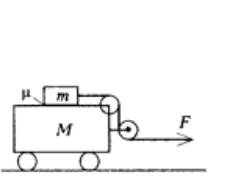
\includegraphics[width=0.9\textwidth]{src/2-picture.png}
        \captionof{figure}{}
      \end{center}  
    \end{minipage}
    \hfill
    \begin{minipage}[t]{0.45\textwidth}
      \begin{center}
        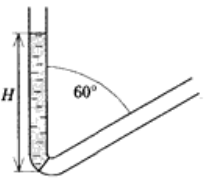
\includegraphics[width=0.9\textwidth]{src/3-picture.png}
        \captionof{figure}{}
      \end{center} 
    \end{minipage}
    
    Ф1555. Тонкая стеклянная трубка, изогнутая в виде буквы V с углом $a = 60^{\circ}$ (рис. 3), закреплена неподнижно. Одно колено трубки отделено от другого закрытым краном. В вертикальное колено наливают воду до весоты $Н$, затем кран открывают, и вода начинает перетекать в другое колено трубки. Считая, что вода не перемешивается и выделения тепла не происходит, найдите пернод происходящего в системе процесса.
    \begin{flushright}\slshapeА.Черноуцан\end{flushright}
    \upshape
    Ф1556. В хорошо откачанный сосуд под поршень ввели некоторое колнчество воды н начали медленно уменьшать объем сосуда, поддерживая постоянную температуру. В таблице приведены давления для нескольких значений объема:
    \begin{center}
      \parbox{0cm}{
        \begin{tabbing}
          \hspace{4em}\= \hspace{2em}\= \hspace{2em}\= \hspace{2em} \= \hspace{2em} \= \hspace{2em}\kill
          \textcolor{yellow}{V,л} \> \colorbox{red}{18} \> \textcolor{yellow}{16} \> \colorbox{red}{14} \> \textcolor{yellow}{12} \> \colorbox{red}{10}\\
          \colorbox{red}{p,кПА} \> \textcolor{yellow}{20} \> \colorbox{red}{23} \> \textcolor{yellow}{24} \> \colorbox{red}{24} \> \textcolor{yellow}{24}\\
        \end{tabbing}} 
    \end{center}
    \begin{spacing}{1.5}
      \hspace{1cm}  Какая температура поддерживалась в этом опыте? При каком значения объема давление внутри сосуда начнет резко возрастать?
     \end{spacing}
    \begin{flushright}\slshapeМ.Учителев\end{flushright}
    \upshape

  \end{minipage}
  \hfill
  \begin{minipage}[t]{0.5\textwidth}
    \hfill
    \begin{center}
      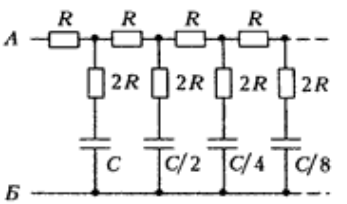
\includegraphics[width=0.55\textwidth]{src/4-picture.png}
      \captionof{figure}{}
    \end{center}
    времени? Какое количество теплоты выделится при этом в резисторе сопротивлением $R$, подключенном к точке $A$?
    \begin{flushright}\slshapeД.Александров\end{flushright}
    Ф1560. На горизонтальной поверхности стола лежит длинный тонкий брусок прямоугольного сечения (рис.5). На один его конец у самого торца намотаны вплотную друг к другу $N$ = 20 витков очень тонкого провода. Магнитное поле с индукцией $В$ = 0,5 Тл направленно вверх, перпендикулярно поверхности стола. Какой величины ток нужно пропустить по проводу, чтобы брусок начал приподниматься? Плотность материала бруска $р$ - $200 кг/м^3$, длина бруска $L$ = 0,1 м.
    \begin{flushright}\slshapeА.Черноуцан\end{flushright}
    \begin{minipage}[t]{0.45\textwidth}
      \begin{center}
        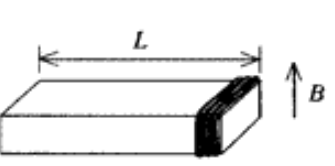
\includegraphics[width=0.9\textwidth]{src/5-picture.png}
        \captionof{figure}{}
      \end{center}  
    \end{minipage}
    \hfill
    \begin{minipage}[t]{0.45\textwidth}
      \begin{center}
        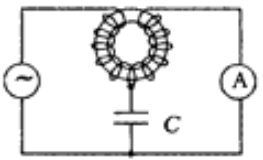
\includegraphics[width=0.9\textwidth]{src/6-picture.png}
        \captionof{figure}{}
      \end{center} 
    \end{minipage}
  \end{minipage}
}
\end{document}